\begin{figure}[H]
    \centering


\tikzset{every picture/.style={line width=0.75pt}} %set default line width to 0.75pt        

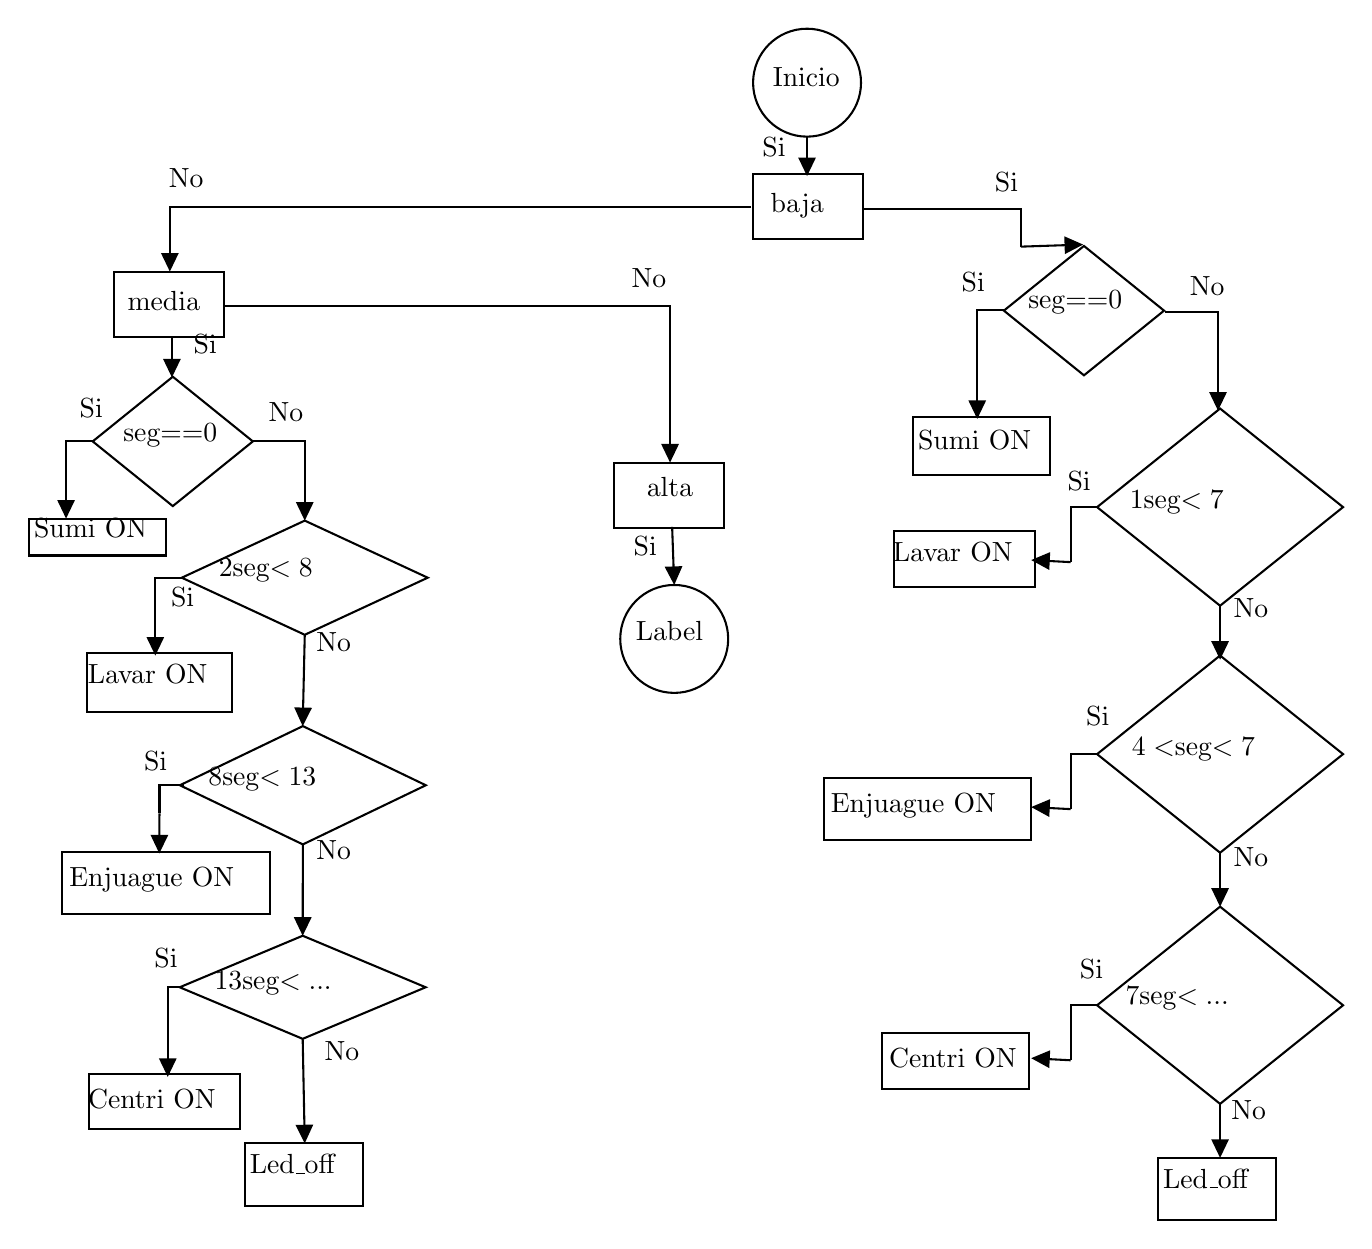
\begin{tikzpicture}[x=0.75pt,y=0.75pt,yscale=-1,xscale=1]
%uncomment if require: \path (0,736); %set diagram left start at 0, and has height of 736

%Flowchart: Connector [id:dp12439739573210629] 
\draw   (355,32) .. controls (355,17.64) and (366.64,6) .. (381,6) .. controls (395.36,6) and (407,17.64) .. (407,32) .. controls (407,46.36) and (395.36,58) .. (381,58) .. controls (366.64,58) and (355,46.36) .. (355,32) -- cycle ;
%Straight Lines [id:da0911199105915208] 
\draw    (381,58) -- (381,74) ;
\draw [shift={(381,77)}, rotate = 270] [fill={rgb, 255:red, 0; green, 0; blue, 0 }  ][line width=0.08]  [draw opacity=0] (8.93,-4.29) -- (0,0) -- (8.93,4.29) -- cycle    ;
%Flowchart: Process [id:dp6149465951989119] 
\draw   (47,123) -- (100,123) -- (100,154.33) -- (47,154.33) -- cycle ;
%Straight Lines [id:da8868380418121589] 
\draw    (74,110) -- (74,120) ;
\draw [shift={(74,123)}, rotate = 270] [fill={rgb, 255:red, 0; green, 0; blue, 0 }  ][line width=0.08]  [draw opacity=0] (8.93,-4.29) -- (0,0) -- (8.93,4.29) -- cycle    ;
%Shape: Right Angle [id:dp6906836722085405] 
\draw   (475.75,141.5) -- (463,141.5) -- (463,168) ;
%Straight Lines [id:da12005298293316646] 
\draw    (463,168) -- (463,191) ;
\draw [shift={(463,194)}, rotate = 270] [fill={rgb, 255:red, 0; green, 0; blue, 0 }  ][line width=0.08]  [draw opacity=0] (8.93,-4.29) -- (0,0) -- (8.93,4.29) -- cycle    ;
%Flowchart: Process [id:dp4261666254360057] 
\draw   (432,193) -- (498,193) -- (498,221) -- (432,221) -- cycle ;
%Straight Lines [id:da019990857102445414] 
\draw    (579,164) -- (579,187) ;
\draw [shift={(579,190)}, rotate = 270] [fill={rgb, 255:red, 0; green, 0; blue, 0 }  ][line width=0.08]  [draw opacity=0] (8.93,-4.29) -- (0,0) -- (8.93,4.29) -- cycle    ;
%Shape: Right Angle [id:dp6724134432403848] 
\draw   (408,93) -- (484,93) -- (484,111) ;
%Straight Lines [id:da7874407775672443] 
\draw    (484,111) -- (511,110.1) ;
\draw [shift={(514,110)}, rotate = 178.09] [fill={rgb, 255:red, 0; green, 0; blue, 0 }  ][line width=0.08]  [draw opacity=0] (8.93,-4.29) -- (0,0) -- (8.93,4.29) -- cycle    ;
%Shape: Right Angle [id:dp1803471909800265] 
\draw   (553.25,142.5) -- (579,142.5) -- (579,164) ;
%Flowchart: Decision [id:dp8940401462112177] 
\draw   (580,189) -- (639.25,236.5) -- (580,284) -- (520.75,236.5) -- cycle ;
%Shape: Right Angle [id:dp9888575078003836] 
\draw   (520.75,236.5) -- (508,236.5) -- (508,263) ;
%Straight Lines [id:da9039594504404762] 
\draw    (508,263) -- (492,262.16) ;
\draw [shift={(489,262)}, rotate = 3.01] [fill={rgb, 255:red, 0; green, 0; blue, 0 }  ][line width=0.08]  [draw opacity=0] (8.93,-4.29) -- (0,0) -- (8.93,4.29) -- cycle    ;
%Flowchart: Process [id:dp1878281348761568] 
\draw   (423,248) -- (491,248) -- (491,275) -- (423,275) -- cycle ;
%Straight Lines [id:da7045473332712788] 
\draw    (580,284) -- (580,307) ;
\draw [shift={(580,310)}, rotate = 270] [fill={rgb, 255:red, 0; green, 0; blue, 0 }  ][line width=0.08]  [draw opacity=0] (8.93,-4.29) -- (0,0) -- (8.93,4.29) -- cycle    ;
%Flowchart: Decision [id:dp7590302190788398] 
\draw   (580,308) -- (639.25,355.5) -- (580,403) -- (520.75,355.5) -- cycle ;
%Shape: Right Angle [id:dp21013725002314598] 
\draw   (520.75,355.5) -- (508,355.5) -- (508,382) ;
%Straight Lines [id:da9648131280624423] 
\draw    (508,382) -- (492,381.16) ;
\draw [shift={(489,381)}, rotate = 3.01] [fill={rgb, 255:red, 0; green, 0; blue, 0 }  ][line width=0.08]  [draw opacity=0] (8.93,-4.29) -- (0,0) -- (8.93,4.29) -- cycle    ;
%Flowchart: Process [id:dp9160651251463305] 
\draw   (389,367) -- (489,367) -- (489,397) -- (389,397) -- cycle ;
%Straight Lines [id:da8522104020423502] 
\draw    (580,403) -- (580,426) ;
\draw [shift={(580,429)}, rotate = 270] [fill={rgb, 255:red, 0; green, 0; blue, 0 }  ][line width=0.08]  [draw opacity=0] (8.93,-4.29) -- (0,0) -- (8.93,4.29) -- cycle    ;
%Flowchart: Decision [id:dp12658023343568292] 
\draw   (580,429) -- (639.25,476.5) -- (580,524) -- (520.75,476.5) -- cycle ;
%Shape: Right Angle [id:dp134629382260554] 
\draw   (520.75,476.5) -- (508,476.5) -- (508,503) ;
%Straight Lines [id:da02925904812151492] 
\draw    (508,503) -- (492,502.16) ;
\draw [shift={(489,502)}, rotate = 3.01] [fill={rgb, 255:red, 0; green, 0; blue, 0 }  ][line width=0.08]  [draw opacity=0] (8.93,-4.29) -- (0,0) -- (8.93,4.29) -- cycle    ;
%Flowchart: Process [id:dp9433679378308446] 
\draw   (417,490) -- (488,490) -- (488,517) -- (417,517) -- cycle ;
%Straight Lines [id:da26870518401603505] 
\draw    (580,524) -- (580,547) ;
\draw [shift={(580,550)}, rotate = 270] [fill={rgb, 255:red, 0; green, 0; blue, 0 }  ][line width=0.08]  [draw opacity=0] (8.93,-4.29) -- (0,0) -- (8.93,4.29) -- cycle    ;
%Flowchart: Process [id:dp9811382267708229] 
\draw   (550,550) -- (607,550) -- (607,580) -- (550,580) -- cycle ;
%Shape: Right Angle [id:dp8598411976781433] 
\draw   (354,92) -- (74,92) -- (74,110) ;
%Flowchart: Decision [id:dp21488379209338482] 
\draw   (75.42,173.67) -- (114,204.83) -- (75.42,236) -- (36.83,204.83) -- cycle ;
%Shape: Right Angle [id:dp26291738895516636] 
\draw   (36.83,204.83) -- (24,204.83) -- (24,216) ;
%Straight Lines [id:da6659896216340511] 
\draw    (24,216) -- (24,239) ;
\draw [shift={(24,242)}, rotate = 270] [fill={rgb, 255:red, 0; green, 0; blue, 0 }  ][line width=0.08]  [draw opacity=0] (8.93,-4.29) -- (0,0) -- (8.93,4.29) -- cycle    ;
%Flowchart: Process [id:dp23715148378192508] 
\draw   (6,242) -- (72,242) -- (72,259.81) -- (6,259.81) -- cycle ;
%Straight Lines [id:da7175092852653877] 
\draw    (139,217) -- (139,240) ;
\draw [shift={(139,243)}, rotate = 270] [fill={rgb, 255:red, 0; green, 0; blue, 0 }  ][line width=0.08]  [draw opacity=0] (8.93,-4.29) -- (0,0) -- (8.93,4.29) -- cycle    ;
%Shape: Right Angle [id:dp7282756797126677] 
\draw   (114,204.83) -- (139,204.83) -- (139,217) ;
%Flowchart: Decision [id:dp679752545363411] 
\draw   (139,243) -- (198.25,270.5) -- (139,298) -- (79.75,270.5) -- cycle ;
%Shape: Right Angle [id:dp8761291449153592] 
\draw   (79.75,270.5) -- (67,270.5) -- (67,297) ;
%Straight Lines [id:da9650771288485256] 
\draw    (67,297) -- (67,305) ;
\draw [shift={(67,308)}, rotate = 270] [fill={rgb, 255:red, 0; green, 0; blue, 0 }  ][line width=0.08]  [draw opacity=0] (8.93,-4.29) -- (0,0) -- (8.93,4.29) -- cycle    ;
%Flowchart: Process [id:dp6312403338347992] 
\draw   (34,306.67) -- (104,306.67) -- (104,335) -- (34,335) -- cycle ;
%Straight Lines [id:da35042274703091447] 
\draw    (139,298) -- (138.07,339) ;
\draw [shift={(138,342)}, rotate = 271.3] [fill={rgb, 255:red, 0; green, 0; blue, 0 }  ][line width=0.08]  [draw opacity=0] (8.93,-4.29) -- (0,0) -- (8.93,4.29) -- cycle    ;
%Flowchart: Decision [id:dp2936421274241927] 
\draw   (138.08,342) -- (197.33,370.5) -- (138.08,399) -- (78.83,370.5) -- cycle ;
%Shape: Right Angle [id:dp42175811220875525] 
\draw   (80.83,370.17) -- (69,370.17) -- (69,384) ;
%Straight Lines [id:da36210638117227556] 
\draw    (69,384) -- (68.93,400.33) ;
\draw [shift={(68.92,403.33)}, rotate = 270.25] [fill={rgb, 255:red, 0; green, 0; blue, 0 }  ][line width=0.08]  [draw opacity=0] (8.93,-4.29) -- (0,0) -- (8.93,4.29) -- cycle    ;
%Flowchart: Process [id:dp06368758111530282] 
\draw   (22.08,402.67) -- (122.08,402.67) -- (122.08,432.67) -- (22.08,432.67) -- cycle ;
%Straight Lines [id:da6829150776274491] 
\draw    (138.08,399) -- (138.01,440) ;
\draw [shift={(138,443)}, rotate = 270.11] [fill={rgb, 255:red, 0; green, 0; blue, 0 }  ][line width=0.08]  [draw opacity=0] (8.93,-4.29) -- (0,0) -- (8.93,4.29) -- cycle    ;
%Flowchart: Decision [id:dp21332806721811415] 
\draw   (138,443) -- (197.25,467.83) -- (138,492.67) -- (78.75,467.83) -- cycle ;
%Shape: Right Angle [id:dp8939949854170095] 
\draw   (78.75,467.83) -- (73,467.83) -- (73,496) ;
%Straight Lines [id:da9774114081951284] 
\draw    (73,496) -- (73,508) ;
\draw [shift={(73,511)}, rotate = 270] [fill={rgb, 255:red, 0; green, 0; blue, 0 }  ][line width=0.08]  [draw opacity=0] (8.93,-4.29) -- (0,0) -- (8.93,4.29) -- cycle    ;
%Flowchart: Process [id:dp775718312939818] 
\draw   (35.08,509.67) -- (108,509.67) -- (108,536) -- (35.08,536) -- cycle ;
%Straight Lines [id:da016170408812257175] 
\draw    (138,492.67) -- (138.94,540) ;
\draw [shift={(139,543)}, rotate = 268.86] [fill={rgb, 255:red, 0; green, 0; blue, 0 }  ][line width=0.08]  [draw opacity=0] (8.93,-4.29) -- (0,0) -- (8.93,4.29) -- cycle    ;
%Flowchart: Decision [id:dp3953876048094218] 
\draw   (514.42,110.67) -- (553,141.83) -- (514.42,173) -- (475.83,141.83) -- cycle ;
%Straight Lines [id:da4743960354930279] 
\draw    (75,155) -- (75,171) ;
\draw [shift={(75,174)}, rotate = 270] [fill={rgb, 255:red, 0; green, 0; blue, 0 }  ][line width=0.08]  [draw opacity=0] (8.93,-4.29) -- (0,0) -- (8.93,4.29) -- cycle    ;
%Shape: Right Angle [id:dp8466659682561892] 
\draw   (100,139.67) -- (315,139.67) -- (315,194) ;
%Straight Lines [id:da4649712336561458] 
\draw    (315,194) -- (315,212) ;
\draw [shift={(315,215)}, rotate = 270] [fill={rgb, 255:red, 0; green, 0; blue, 0 }  ][line width=0.08]  [draw opacity=0] (8.93,-4.29) -- (0,0) -- (8.93,4.29) -- cycle    ;
%Flowchart: Process [id:dp8283630291095716] 
\draw   (288,215.33) -- (341,215.33) -- (341,246.67) -- (288,246.67) -- cycle ;
%Flowchart: Process [id:dp4922525180421693] 
\draw   (355,76) -- (408,76) -- (408,107.33) -- (355,107.33) -- cycle ;
%Straight Lines [id:da28645691514326366] 
\draw    (316,246) -- (316.89,271) ;
\draw [shift={(317,274)}, rotate = 267.95] [fill={rgb, 255:red, 0; green, 0; blue, 0 }  ][line width=0.08]  [draw opacity=0] (8.93,-4.29) -- (0,0) -- (8.93,4.29) -- cycle    ;
%Flowchart: Connector [id:dp6291119086530925] 
\draw   (291,300) .. controls (291,285.64) and (302.64,274) .. (317,274) .. controls (331.36,274) and (343,285.64) .. (343,300) .. controls (343,314.36) and (331.36,326) .. (317,326) .. controls (302.64,326) and (291,314.36) .. (291,300) -- cycle ;
%Flowchart: Process [id:dp4549925468032834] 
\draw   (110,543) -- (167,543) -- (167,573) -- (110,573) -- cycle ;

% Text Node
\draw (363,23) node [anchor=north west][inner sep=0.75pt]   [align=left] {Inicio};
% Text Node
\draw (362,84) node [anchor=north west][inner sep=0.75pt]   [align=left] {baja};
% Text Node
\draw (302.33,220.67) node [anchor=north west][inner sep=0.75pt]   [align=left] {alta};
% Text Node
\draw (52.14,130.97) node [anchor=north west][inner sep=0.75pt]   [align=left] {media};
% Text Node
\draw (433,198) node [anchor=north west][inner sep=0.75pt]   [align=left] {Sumi ON};
% Text Node
\draw (72,72) node [anchor=north west][inner sep=0.75pt]   [align=left] {No};
% Text Node
\draw (564,124) node [anchor=north west][inner sep=0.75pt]   [align=left] {No};
% Text Node
\draw (505,218) node [anchor=north west][inner sep=0.75pt]   [align=left] {Si};
% Text Node
\draw (358,57) node [anchor=north west][inner sep=0.75pt]   [align=left] {Si};
% Text Node
\draw (454,122) node [anchor=north west][inner sep=0.75pt]   [align=left] {Si};
% Text Node
\draw (535,227) node [anchor=north west][inner sep=0.75pt]   [align=left] {$\displaystyle 1\leqslant $seg$\displaystyle < 7$};
% Text Node
\draw (412,252) node [anchor=north west][inner sep=0.75pt]   [align=left] { \ \ Lavar ON};
% Text Node
\draw (585,279) node [anchor=north west][inner sep=0.75pt]   [align=left] {No};
% Text Node
\draw (536,346) node [anchor=north west][inner sep=0.75pt]   [align=left] {$\displaystyle 4< $seg$\displaystyle < 7$};
% Text Node
\draw (391,373) node [anchor=north west][inner sep=0.75pt]   [align=left] {Enjuague ON};
% Text Node
\draw (514,331) node [anchor=north west][inner sep=0.75pt]   [align=left] {Si};
% Text Node
\draw (585,399) node [anchor=north west][inner sep=0.75pt]   [align=left] {No};
% Text Node
\draw (533,466) node [anchor=north west][inner sep=0.75pt]   [align=left] {$\displaystyle 7\leqslant $seg$\displaystyle < ...$};
% Text Node
\draw (419,496) node [anchor=north west][inner sep=0.75pt]   [align=left] {Centri ON};
% Text Node
\draw (511,453) node [anchor=north west][inner sep=0.75pt]   [align=left] {Si};
% Text Node
\draw (584,521) node [anchor=north west][inner sep=0.75pt]   [align=left] {No};
% Text Node
\draw (551,554) node [anchor=north west][inner sep=0.75pt]   [align=left] {Led\_off};
% Text Node
\draw (50.08,194.67) node [anchor=north west][inner sep=0.75pt]   [align=left] {seg==0};
% Text Node
\draw (7.08,240.5) node [anchor=north west][inner sep=0.75pt]   [align=left] {Sumi ON};
% Text Node
\draw (120.08,184.67) node [anchor=north west][inner sep=0.75pt]   [align=left] {No};
% Text Node
\draw (73.08,273.67) node [anchor=north west][inner sep=0.75pt]   [align=left] {Si};
% Text Node
\draw (29.08,182.67) node [anchor=north west][inner sep=0.75pt]   [align=left] {Si};
% Text Node
\draw (96.08,259.67) node [anchor=north west][inner sep=0.75pt]   [align=left] {$\displaystyle 2\leqslant $seg$\displaystyle < 8$};
% Text Node
\draw (24.08,310.67) node [anchor=north west][inner sep=0.75pt]   [align=left] { \ \ Lavar ON};
% Text Node
\draw (143.08,295.67) node [anchor=north west][inner sep=0.75pt]   [align=left] {No};
% Text Node
\draw (91.08,360.67) node [anchor=north west][inner sep=0.75pt]   [align=left] {$\displaystyle 8\leqslant $seg$\displaystyle < 13$};
% Text Node
\draw (24.08,408.67) node [anchor=north west][inner sep=0.75pt]   [align=left] {Enjuague ON};
% Text Node
\draw (60.08,352.67) node [anchor=north west][inner sep=0.75pt]   [align=left] {Si};
% Text Node
\draw (143.08,395.67) node [anchor=north west][inner sep=0.75pt]   [align=left] {No};
% Text Node
\draw (94.08,458.67) node [anchor=north west][inner sep=0.75pt]   [align=left] {$\displaystyle 13\leqslant $seg$\displaystyle < ...$};
% Text Node
\draw (33.08,515.67) node [anchor=north west][inner sep=0.75pt]   [align=left] {Centri ON};
% Text Node
\draw (65.08,447.67) node [anchor=north west][inner sep=0.75pt]   [align=left] {Si};
% Text Node
\draw (147.08,492.67) node [anchor=north west][inner sep=0.75pt]   [align=left] {No};
% Text Node
\draw (486.08,130.67) node [anchor=north west][inner sep=0.75pt]   [align=left] {seg==0};
% Text Node
\draw (297,290) node [anchor=north west][inner sep=0.75pt]   [align=left] {Label};
% Text Node
\draw (111,547) node [anchor=north west][inner sep=0.75pt]   [align=left] {Led\_off};
% Text Node
\draw (470,74) node [anchor=north west][inner sep=0.75pt]   [align=left] {Si};
% Text Node
\draw (84,152) node [anchor=north west][inner sep=0.75pt]   [align=left] {Si};
% Text Node
\draw (295,120) node [anchor=north west][inner sep=0.75pt]   [align=left] {No};
% Text Node
\draw (296,249) node [anchor=north west][inner sep=0.75pt]   [align=left] {Si};


\end{tikzpicture}

\caption{Máquina de estados transición de LEDs.}
\label{sch3}
\end{figure}